\documentclass[a4paper,10pt]{article}
\usepackage[utf8]{inputenc}

\usepackage{graphicx}


%opening
\title{3D Reconstruction using Affine-Invariant Keypoints}
\author{}

\begin{document}

\maketitle

\begin{abstract}
In this report we describe our work on 3D reconstruction using affine-invariant keypoints.
The system consists of a number of stages, each of which has been described in detail in previous reports.
Here we will limit ourselves to a high-level conceptual overview of the pipeline, a walkthrough of our code and a detailed description of newly implemented algorithms and results.

\end{abstract}

\section{Feature Detection \& Description}
Keypoints are detected in all images using both Hessian-affine and Harris-affine region detectors.
These detectors are very similar, the difference being that Harris-affine uses the second moment matrix (as described in our previous report), while Hessian-affine uses the Hessian. CITE
For every point we precompute a SIFT descriptor, which is saved to disk.
These descriptors can then be matched between views, but a naive matching procedure will result in many false matches.
In the following section, we discuss how to remedy this using a RANSAC-based robust estimation of the fundamental matrix, which enables us to discard inconsistent matches.

\section{Epipolar Geometry}

In general one cannot find a distance treshold for SIFT descriptor-matching such that all correct and no incorrect matches are found.
We will therefor not attempt to find the best threshold setting, but instead rely on a rather lenient setting and remove false matches in a subsequent stage.
The idea is to use a RANSAC-based robust estimation procedure to estimate the epipolar geometry of the setup, and to use this to discard those matches that do not respect the epipolar constraints (i.e. the RANSAC outliers).

Our RANSAC algorithm (\verb+estimateFundamental.m+) performs robust estimation of the fundamental matrix $F$ (employing the normalized eight-point algorithm, as described in a previous report), but in our case we are solely interested in the set of inliers; $F$ itself is discarded.

\section{Chaining \& Stitching}
\subsection{The point-view matrix}
For long video sequences, it is unlikely that a single point remains visible in all frames.
In order to still be able to perform 3D reconstruction on such sequences, we must determine the visibility of each point in each frame.
Often, the presence of point $i$ in view $j$ is indicated by a value of $1$ in entry $M_{ij}$ of the point-view matrix $M$.
In our implementation (\verb+chainImages.m+), we do not store a binary matrix but instead store a matrix of indices into the cell-matrix of features.
This feature matrix stores the 2D coordinates, as well as the descriptor.

The point-view matrix has views in the rows, and points in the columns.
It is constructed as follows.
The RANSAC procedure described in the previous section is applied to consecutive frames in the sequence, mod $N$ (where $N$ is the number of frames).
For the first pair, we simply add the indices of matched points to the same column of the first two rows of the point-view matrix.
For subsequent frame-pairs, we perform set-intersection on the sets of feature-indices of current and previous frames, in order to track points over time.
The very last frame-pair, consisting of the last and first frames, requires special treatment.
After adding `new' matches found in the last frame, we move the matches of points that also match the first frame over to the columns that had already been allocated to those points in the first frame.
Obviously, this process will only work for circular sequences, but this is easily enforced and only required during model-building.

\subsection{Tomasi-Kanade factorization}
Given a point-view matrix, we can select dense blocks from it, and perform 3D reconstruction on each block.
This is implemented in \verb+TomasiKanadeFactorization.m+, a detailed explanation of which can be found in our previous report.
The result is a number of point clouds, each one containing points that also occur in other clouds.
These clouds however are not aligned, due to the fact that the factorization can only recover structure up to an affine warp.
Since the composition of affine transformations is affine (invertible affine transformations form a group), the individual clouds are affinely related to each other.


\subsection{Procrustes analysis}

In order to align the clouds and to retrieve the true Euclidean structure, we can proceed in two ways.
One way is to use an affine version of procrustes analysis to align the clouds and then perform a Euclidean upgrade by optimizing for unit orthogonal camera axes.
A much simpler approach is to first perform the Euclidean upgrade, making use of only one dense block at a time, and to then use a standard Euclidean procrustes analysis to align the clouds.
As can be seen in section \ref{sec:vis}, this works very well.

Procrustes analysis itself is just a fancy name for the estimation of a suitably constrained linear transformation that optimally aligns point clouds.
In our case we require the transformation to be a similarity transformation (that may or may not be continuously connected to the identity).
We successively align each cloud to a combined cloud, which is initialized to the first cloud.
The alignment is performed by minimization with respect to the transformation, of the sum of the squared distance between the points that the merged cloud and to-be-aligned cloud have in common.
We found that an iterative optimization of the reference shape (`generalized procrustes analysis') was not necessary.

\section{Visualization}
\label{sec:vis}
The result of the core algorithm is a 3D point cloud, as shown in figure \ref{fig:clouds}.
To improve on this visualization, we created a surface rendering using MATLAB's \verb+surf+ command, as suggested in the assignment.
This works well for most viewing angles for the house model, but for the teddy bear model, this approach is problematic.
Mathematically, points do not have an area and so occlusion cannot be established directly from point clouds.
Since \verb+surf+ uses all points in the cloud, the rendered surface will be highly affected by points that would have been occluded in the real scene.

\begin{figure}[ht]
\caption{Output of the 3D reconstruction algorithm}
\begin{minipage}[b]{0.45\linewidth}
\centering
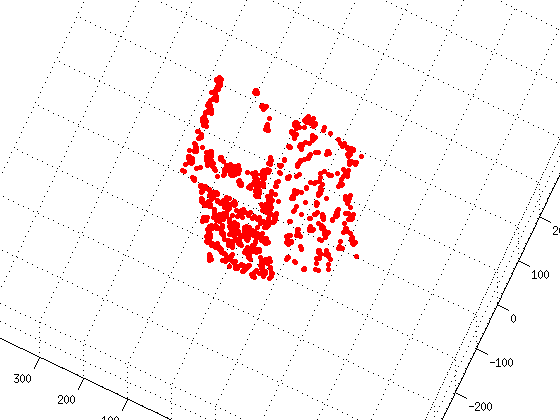
\includegraphics[width=\textwidth]{cloud_house1}
\caption{House model}
\label{fig:figure1}
\end{minipage}
\hspace{0.5cm}
\begin{minipage}[b]{0.45\linewidth}
\centering
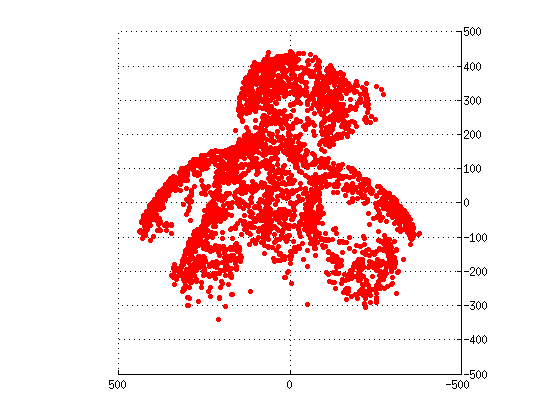
\includegraphics[width=\textwidth]{cloud_teddy1}
\caption{Teddy bear model}
\label{fig:figure2}
\end{minipage}
\label{fig:clouds}
\end{figure}

As a rudimentary solution, we computed the viewing direction and used it as the surface normal for a clipping plane placed at the center of mass of the point cloud.
Points behind the plane, as seen from the camera are discarded for visualization purposes.

As a little bonus, we mapped the texture on the object by projecting every point on the surface to the camera plane as recovered in the structure-motion factorization, and using the projected coordinates in a texture lookup.
This is simplest for the first frame, which is not affected by the procrustes analysis, but other viewing directions could easily be textured by first transforming from world coordinates to camera coordinates using the inverse of the procrustes-transformation.
Textured objects are shown in figure REF.

\begin{figure}[ht]
\begin{minipage}[b]{0.45\linewidth}
\centering
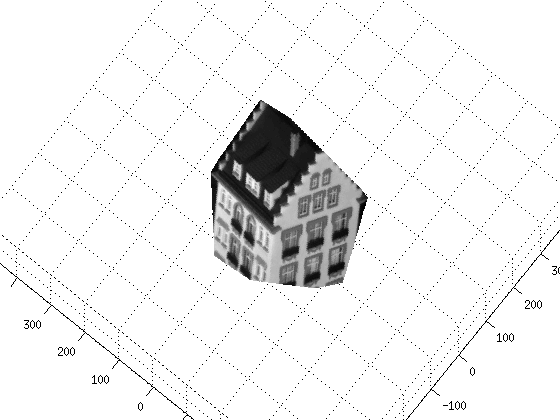
\includegraphics[width=\textwidth]{textured_house1}
\caption{default}
\label{fig:figure1}
\end{minipage}
\hspace{0.5cm}
\begin{minipage}[b]{0.45\linewidth}
\centering
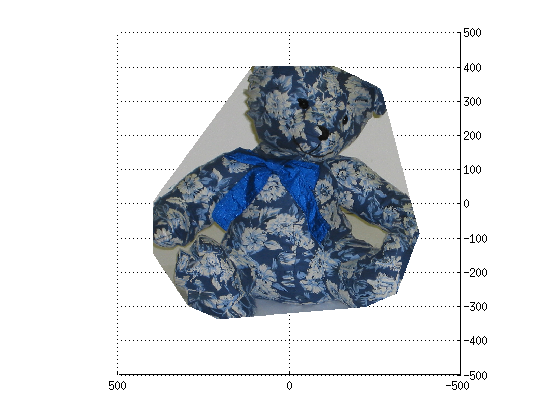
\includegraphics[width=\textwidth]{textured_teddy1}
\caption{default}
\label{fig:figure2}
\end{minipage}
\end{figure}

\end{document}
